\documentclass[12pt]{article}
\usepackage[brazil]{babel}
\usepackage[T1]{fontenc}
\usepackage[utf8]{inputenc}
\usepackage{amssymb}
\usepackage[pdftex]{graphicx}
\usepackage{listings}
\usepackage{amsmath}
\usepackage{float}


\begin{document}
\title{Introdução à Física Computacional \\ Projeto 5}
\author{Luiz Fernando S. E. Santos\\No. USP 10892680}
\date{Junho de 2019}
\maketitle

\pagebreak

\section{Introdução}
\mbox{}

Na seguinte prática, utilizamos de diversos algoritmos computacionais para o estudo de mapas logísticos, caos determinístico e dinâmica populacional. 
No primeiro exercício, trabalhamos com o um mapa logístico com um ponto fixo de período um. Já no segundo com dobras de período, o que nos leva ao caos deterministico e o aparecimento de fractais.
No terceiro exercício, estudamos o modelo predador-presa de Lotka-Volterra, bem como utilizamos o já apresentado método de Runge-Kutta de ordem 4 para sua integação numérica.

Os programas do projeto foram feitos em C++, ao passo que o Python 3.5.2 com as bibliotecas Numpy e Matplotlib foi usado para graficar os resultados e, em alguns casos, facilitar algumas manipulações com os conjuntos de dados ao usar a estrutura de arrays do Numpy.

\section{Instruções}
\mbox{}

Para a compilação dos programas .cpp, estando na pasta com o programa desejado deve-se executar no terminal:

\begin{lstlisting}[language = bash]
g++ nomedoarquivo.cpp -o nomedoarquivo
\end{lstlisting}

Um arquivo \textit{nomedoarquivo} será gerado. Para executá-lo, basta digitar também no terminal:

\begin{lstlisting}[language = bash]
./nomedoarquivo
\end{lstlisting}

Os programas .cpp em geral já possuem um script para gerar um .dat com os resultados, bem como plotar e mostrar o gráfico deles com o .py. Caso hajam os resultados e se deseje executar apenas o .py, basta fazer:

\begin{lstlisting}[language = bash]
python3 nomedoarquivo.py
\end{lstlisting}

Desta forma, podem ser testados vários valores iniciais das variáveis, sem a necessidade de plotá-los em um programa externo toda vez que novos dados são gerados. Para alterar esses valores, basta fazer isso no código .cpp, onde eles são atribuídos às tais variáveis.

\section{Métodos e resultados}
\subsection{Ponto fixo de período um}
\subsubsection{(a)}
\mbox{}

Em um programa C++, defino a função:

\begin{equation}
G(x, r) = rx(1 - x)
\end{equation}

E para os valores de $r$ $0.5$, $1.0$, $2.0$, é calculado $f(x) = x$ e $G(x, r)$. Os resultados podem ser visualisados no gráfico:

\begin{figure}[H]
\centering
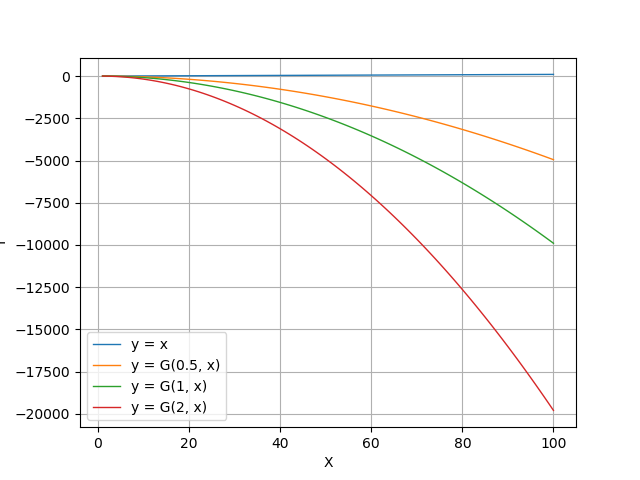
\includegraphics[scale=0.9]{/home/russo/Intro_Fiscomp/P5/1/a/GX.png}
\caption{Funções G e f}
\label{fig1}
\end{figure}

Para entendermos porque da existência da solução não-trivial para a igualdade 

\begin{equation}
G(x, r) = f(x)
\end{equation}

apenas para $r > 1$, podemos desenovolver a equação [2]:

\begin{align*}
rx(1-x) = x\\
r - rx = 1\\
r = \frac{1}{1 - x}
\end{align*}

Supondo $r \leq 1$, teremos que:

\begin{align*}
1 - x \geq 1\\
\Rightarrow x \leq 0
\end{align*}

Mas se $x < 0$, $x \notin ]0, 1[$, como fora definido. Desta forma, o único valor de $x$ que satisfaz [2] para $r < 1$ é $x = 0$ (solução trivial).

\subsubsection{(b)}
\mbox{}

Agora, usando $r = 1, 2, 2.5$, fazemos o mapa logístico para diferentes valores de $x_{0}$. Obtemos, para cada valor de $r$, os seguintes resultados:

\begin{figure}[H]
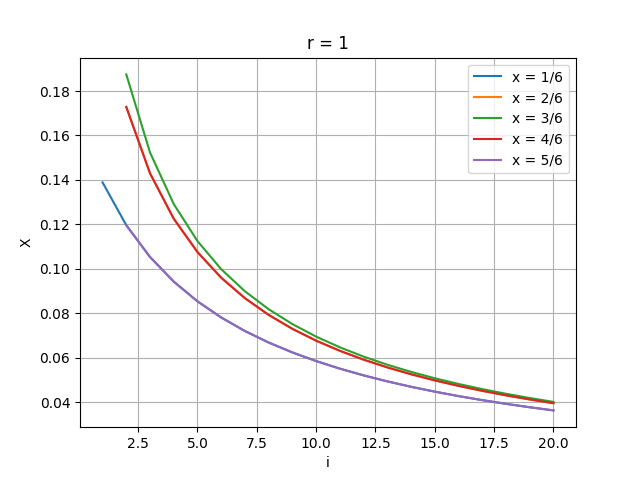
\includegraphics[scale = 0.5]{/home/russo/Intro_Fiscomp/P5/1/b/r1.png}
\includegraphics[scale = 0.5]{/home/russo/Intro_Fiscomp/P5/1/b/r2.png}
\end{figure}
\begin{figure}[H]
\centering
\includegraphics[scale = 0.7]{/home/russo/Intro_Fiscomp/P5/1/b/r25.png}
\caption{gráficos de x contra i}
\label{fig 2}
\end{figure}

Podemos ver claramente que, mesmo para diferentes valores de $x_{0}$, $x$ sempre converge para um valor fixo (valor este que muda de acord com $r$).

\subsubsection{(c)}
\mbox{}

Tomamos agora um $\epsilon << 1$, o qual será usado para obtermos um valor muito próximo de $x_{0}$ ($x_{0} + \epsilon$). Iremos iterar estes dois valores iniciais de $x$ e ver como a distância $d$ entre eles se comporta ao longo das iterações.
Fazendo isso para $\epsilon = 0.01$ e três valores distintos de $r$, $r = 1.5, 2.5, 2.7$, plotamos o gráfico de $d$ contra o índice $i$ da iteração, assim obtendo:

\begin{figure}[H]
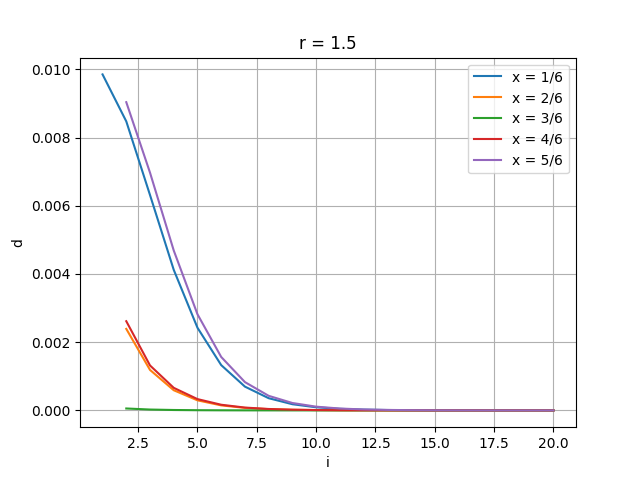
\includegraphics[scale = 0.5]{/home/russo/Intro_Fiscomp/P5/1/c/r15.png}
\includegraphics[scale = 0.5]{/home/russo/Intro_Fiscomp/P5/1/c/r25.png}
\end{figure}
\begin{figure}[H]
\centering
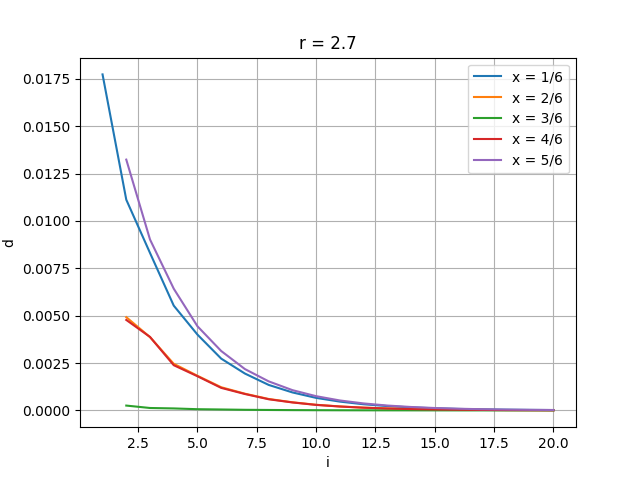
\includegraphics[scale = 0.7]{/home/russo/Intro_Fiscomp/P5/1/c/r27.png}
\caption{gráficos de d contra i}
\label{fig 3}
\end{figure}

Estas curvas encontradas parecem razoávelmente um decaimento exponencial, e podemos confirmar que elas de fato o são ao plotarmos os dados em escala \textit{log-linear}:

\begin{figure}[H]
\centering
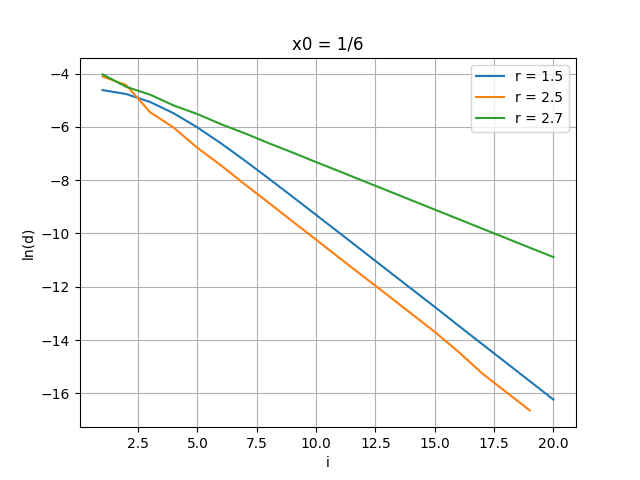
\includegraphics[scale=0.8]{/home/russo/Intro_Fiscomp/P5/1/c/confirmexp.png}
\caption{plot em escala log-lin.}
\label{fig 4}
\end{figure}

Sendo o coef. de Lyapunov $\lambda$ dado pela relação:

\begin{equation}
d_{i} \sim e^{-\lambda i}
\end{equation}

Podemos obtê-lo através do coeficiente ângular ao ajustarmos uma reta no gráfico de $ln(d_{i})$ contra $i$, para cada valor de $r$. Utilizando o programa QtiPlot para isso, obtemos:

\begin{figure}[H]
\centering
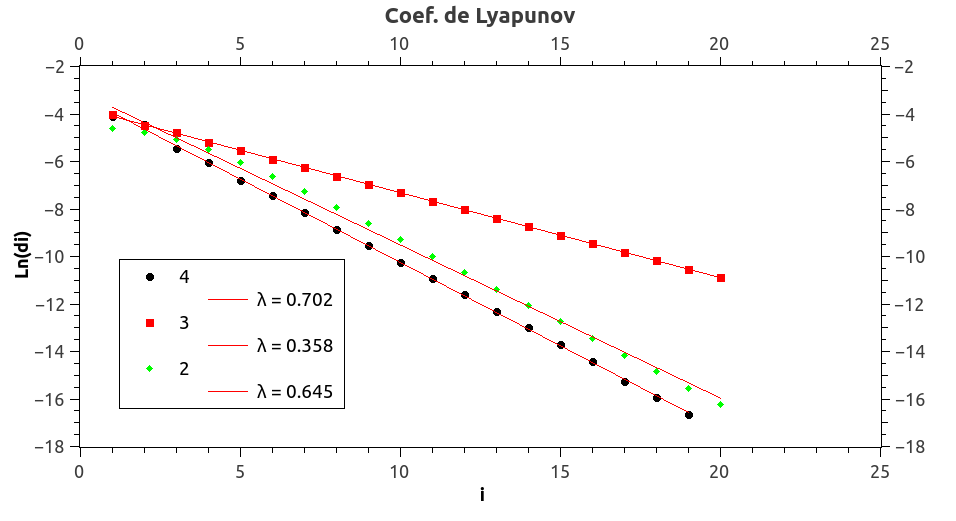
\includegraphics[scale=0.5]{/home/russo/Intro_Fiscomp/P5/1/c/lyapunov.png}
\caption{coef de Lyapunov para cada valor de $r$. Os pontos verdes, pretos e vermelhos correspondem a $r = 1.5, 2.5$ e $2.7$, respectivamente.}
\label{fig 5}
\end{figure}

Podemos checar que isso continua valendo mesmo para os demais valores de $x_{0}$:

\begin{figure}[H]
\centering
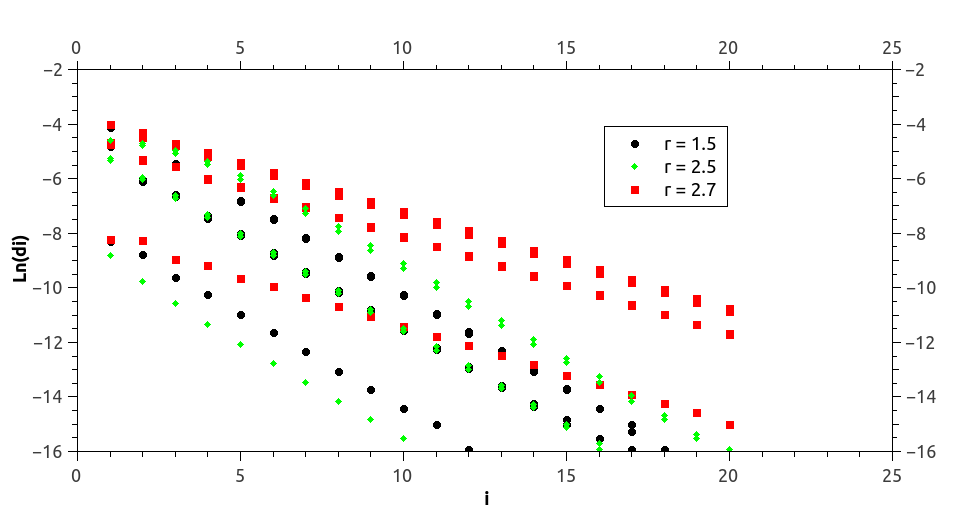
\includegraphics[scale=0.5]{/home/russo/Intro_Fiscomp/P5/1/c/paralels.png}
\caption{retas para os demais valores de $x_{0}$. Podemos ver que elas são paralelas para um mesmo valor de $r$.}
\label{fig 6}
\end{figure}

Pelos resultados vemos que, embora o coeficiente independa de $x_{0}$ neste caso, ele varia com $r$.

\subsubsection{(d)}
\mbox{}

Agora, calculamos o coeficiente de Lyapunov através da estimativa:

\begin{equation}
\lambda \equiv \frac{1}{n}\sum_{j = 0}^{n-1} \ln{|G'(x_{j})|}
\end{equation}

Antes de tudo devemos calcular a primeira derivada de $G(x)$:

\begin{align*}
G'(x) = \frac{d}{dx}rx(1 - x) = r(1 - 2x)
\end{align*}

Tendo isso, iteramos $G(x)$, calculando o logaritmo natural do módulo de sua primeira derivada em cada iteração e adicionando à somatória. Ao fim, dividimos tudo pelo número de iterações $n$. Para alguns diferentes valores de $x_{0}$ obtemos:

\begin{figure}[H]
\centering
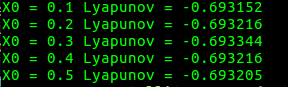
\includegraphics[scale=1]{/home/russo/Intro_Fiscomp/P5/1/d/values.png}
\caption{Valores obtidos para o coef. de Lyapunov através da somatória para diferentes valores de $x_{0}$, com $r = 2.5$.}
\label{fig 7}
\end{figure}

Podemos observar o coeficiente obtido através desse método está razoávelmente próximo daquele que calculamos através do coef. angular da reta ajustada, e de fato ele se mantém estável para diferentes valores de $x_{0}$.

\subsubsection{(e)}
\mbox{}

Tomamos $r = 2.9$ e $x_{0} = 0.1$. Primeiramente fazemos um gráfico de $\ln{|G'(x_{j})|}$ contra $j$ para observar o comportamente do termo dentro da somatória definida anteriormente ao longo das iterações. Desta forma, obtemos o gráfico:

\begin{figure}[H]
\centering
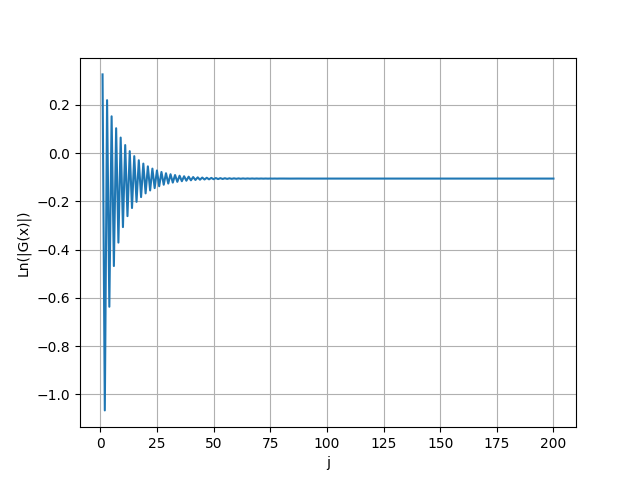
\includegraphics[scale=0.7]{/home/russo/Intro_Fiscomp/P5/1/e/graf.png}
\caption{Varião do logaritmo da derivada com as iterações.}
\label{fig 8}
\end{figure}

Podemos observar que no começo há uma oscilação, enquanto $\ln{|G'(x_{j})|}$ se aproxima de $\lambda$. Após um certo número de iterações, o logaritmo se mantém praticamente constante. Por conta disso, podemos usar a relação [4] e obtemos, para um $j$ grande:

\begin{align*}
\lambda = \frac{1}{n}\sum_{j = 0}^{n-1} \ln{|G'(x_{j})|} 
\approx \frac{n\ln{|G'(x_{j})|}}{n} \\
= \ln{|G'(x_{j})|}
\end{align*}

Para obtermos $\lambda$ desta forma, iteramos a função $100$ vezes, para que o citado termo se mantenha razoávelmente constante. Após, salvamos os valores de $\ln{|G'(x_{j})|}$ em um arquivo. 
Em outro programa .py, lemos este arquivo, salvando os valores obtidos como elementos de um \textit{array}. Contamos a frequência de cada elemento e através disso fazemos um histograma.

Do histograma podemos tirar algumas informações: o valor de $\lambda$ é a média poderada de cada valor de $\ln{|G'(x_{j})|}$ levando em conta sua frequência, ao passo que o erro é obtido através do desvio padrão.

Usando este método, podemos obter dois tipos de resultados para duas situações:
Primeiro, caso a precisão de nossos números não seja tão "grande", obtemos um histograma com poucos valroes diferentes de $\ln{|G'(x_{j})|}$, sendo a maior parte deles com uma frequência muito baixa e um em específico tendo um grande pico:

\begin{figure}[H]
\centering
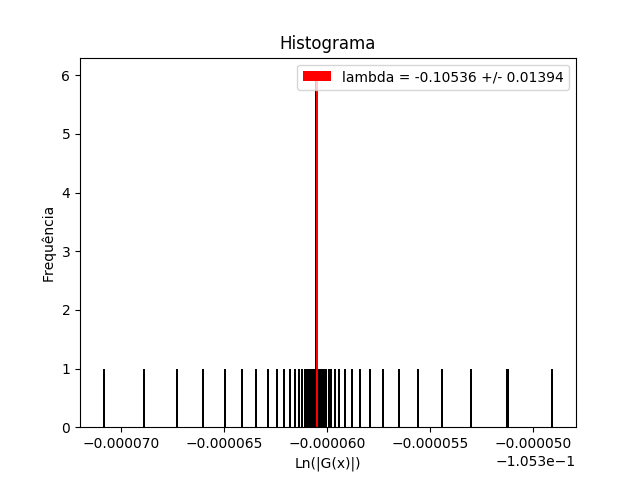
\includegraphics[scale=0.7]{/home/russo/Intro_Fiscomp/P5/1/e/histo1.png}
\caption{Primeiro caso de histograma: precisão da ordem de $10^{-9}$ casas decimais.}
\label{fig 9}
\end{figure}

Já no caso de termos uma precisão muito alta, vamos ter vários valores de $\ln{|G'(x_{j})|}$ com uma frequência baixa, mas com a grande maioria deles se concentrando próximo de $\lambda$:

\begin{figure}[H]
\centering
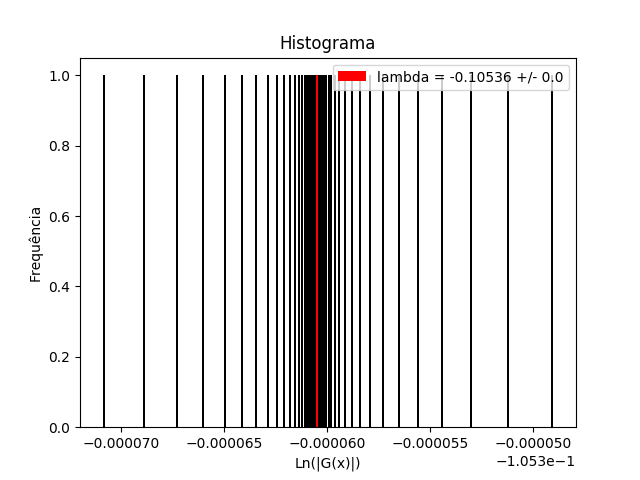
\includegraphics[scale=0.7]{/home/russo/Intro_Fiscomp/P5/1/e/histo2.png}
\caption{Segundo caso de histograma: precisão da ordem de $10^{-14}$ casas decimais.}
\label{fig 10}
\end{figure}

Nosso método funciona bem para ambos os casos, e como o esperado nos dá resultados equivalentes.

\subsection{Dobras de período e caos}

\subsubsection{(a)}
\mbox{}

Sendo $G$ como definido anteriormente, plotamos para $r = 2.9, 3, 3.1$ os gráficos de $f(x) = x$, $g^{2}(x, r) = G(G(x))$. Obtemos:

\begin{figure}[H]
\centering
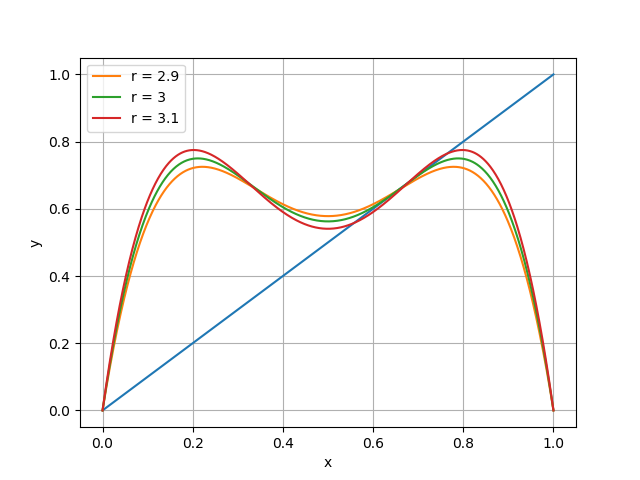
\includegraphics[scale=0.4]{/home/russo/Intro_Fiscomp/P5/2/a/ex2a.png}
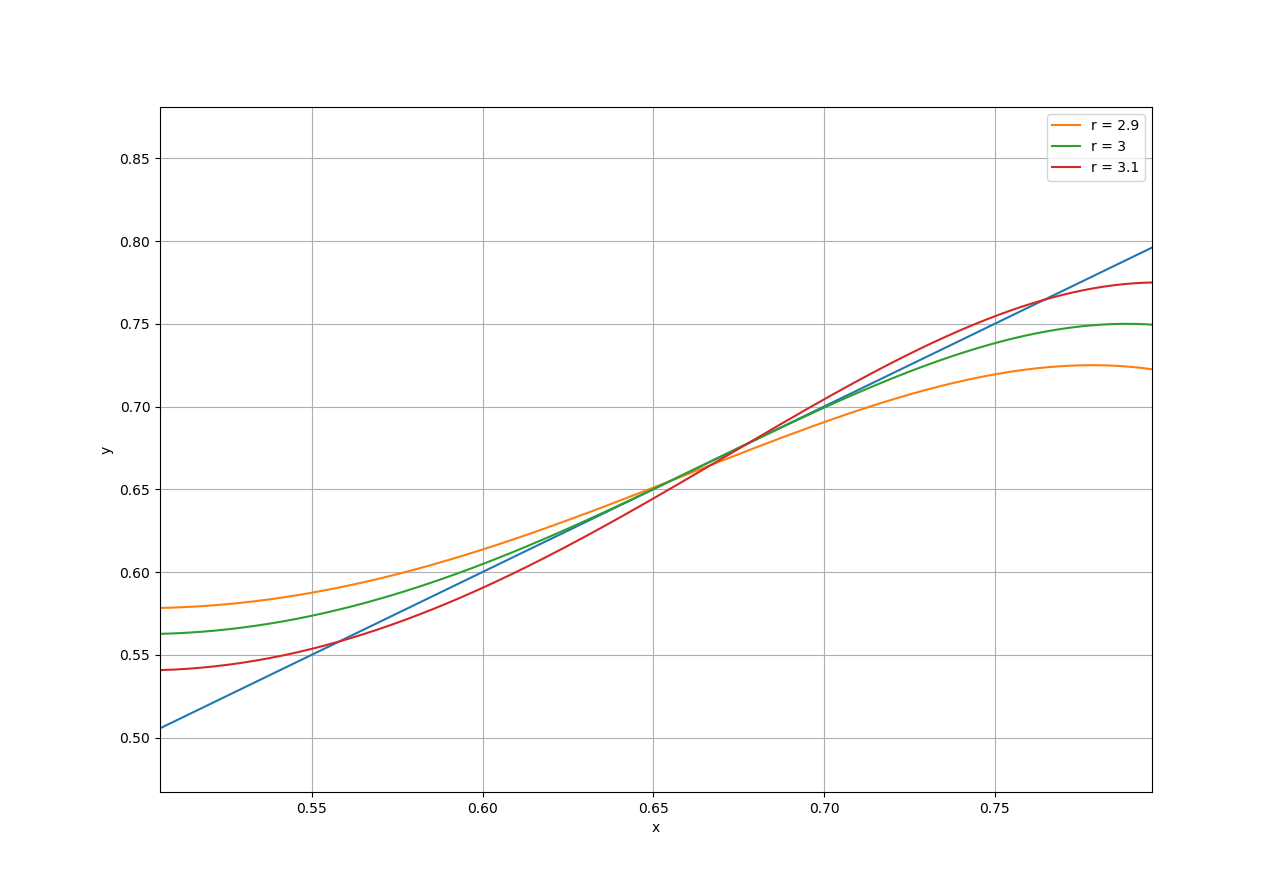
\includegraphics[scale=0.4]{/home/russo/Intro_Fiscomp/P5/2/a/roots.png}

\caption{Plot de $f(x)$ e $g^{2}(x, r)$ para dados valores de $r$.}
\label{fig 11}
\end{figure}

Podemos ver que $f(x)$ e $g^{2}(x, r)$ se interceptam três vezes (além de em $0$) quanto $r = 3.1$.

\subsubsection{(b)}
\mbox{}

Variando $r$ e iterando a equação, visando encontrar o(s) ponto(s) fixo(s) $x^{*}$ para cada valor, podemos plotar um gráfico de $r$ contra $x^{*}$:

\begin{figure}[H]
\centering
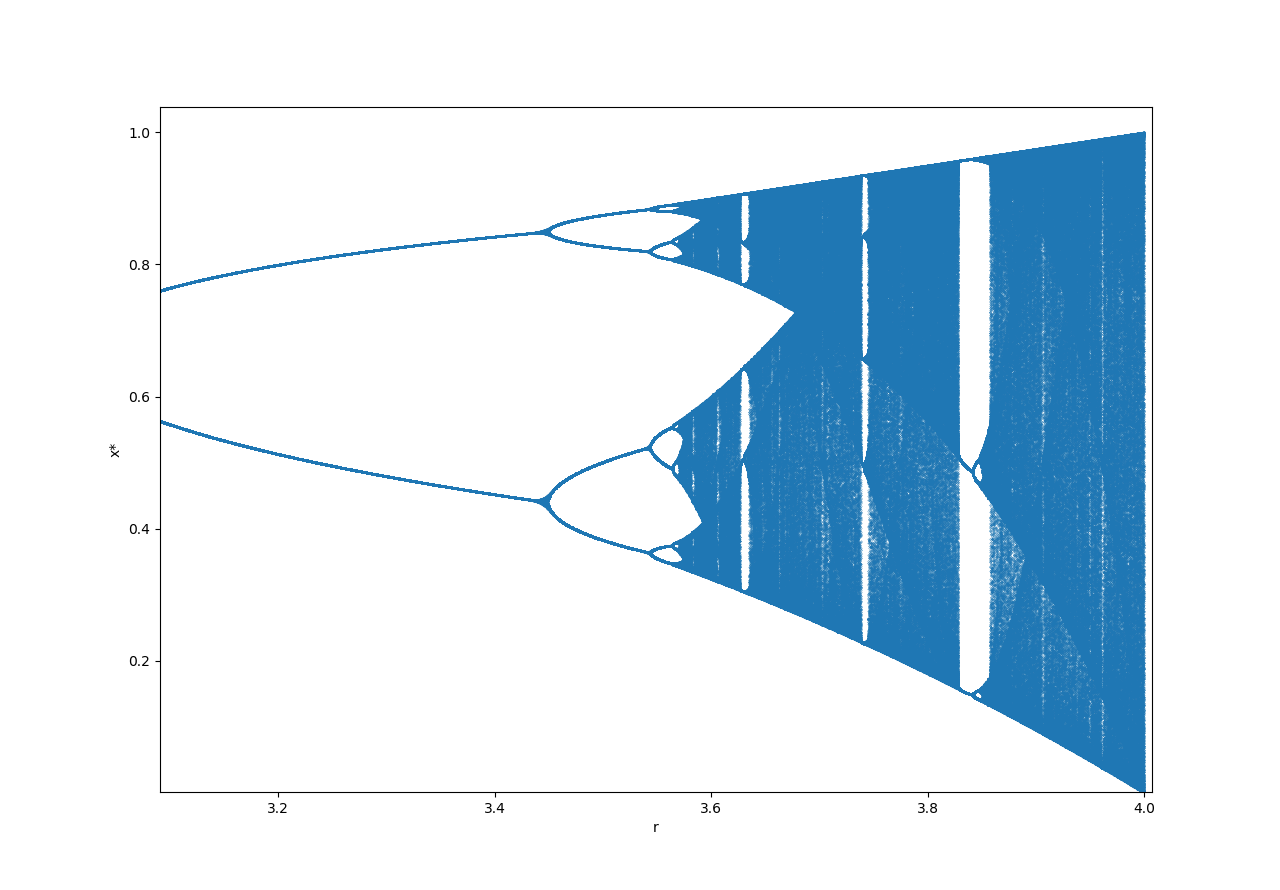
\includegraphics[scale=0.32]{/home/russo/Intro_Fiscomp/P5/2/b/frac2.png}
\caption{Diagrama de bifurcação.}
\label{fig 12}
\end{figure}

É interessante notarmos o comportamento fractal desse diagrama: se dermos um zoom em algum ponto no meio deste diagrama, podemos ver:

\begin{figure}[H]
\centering
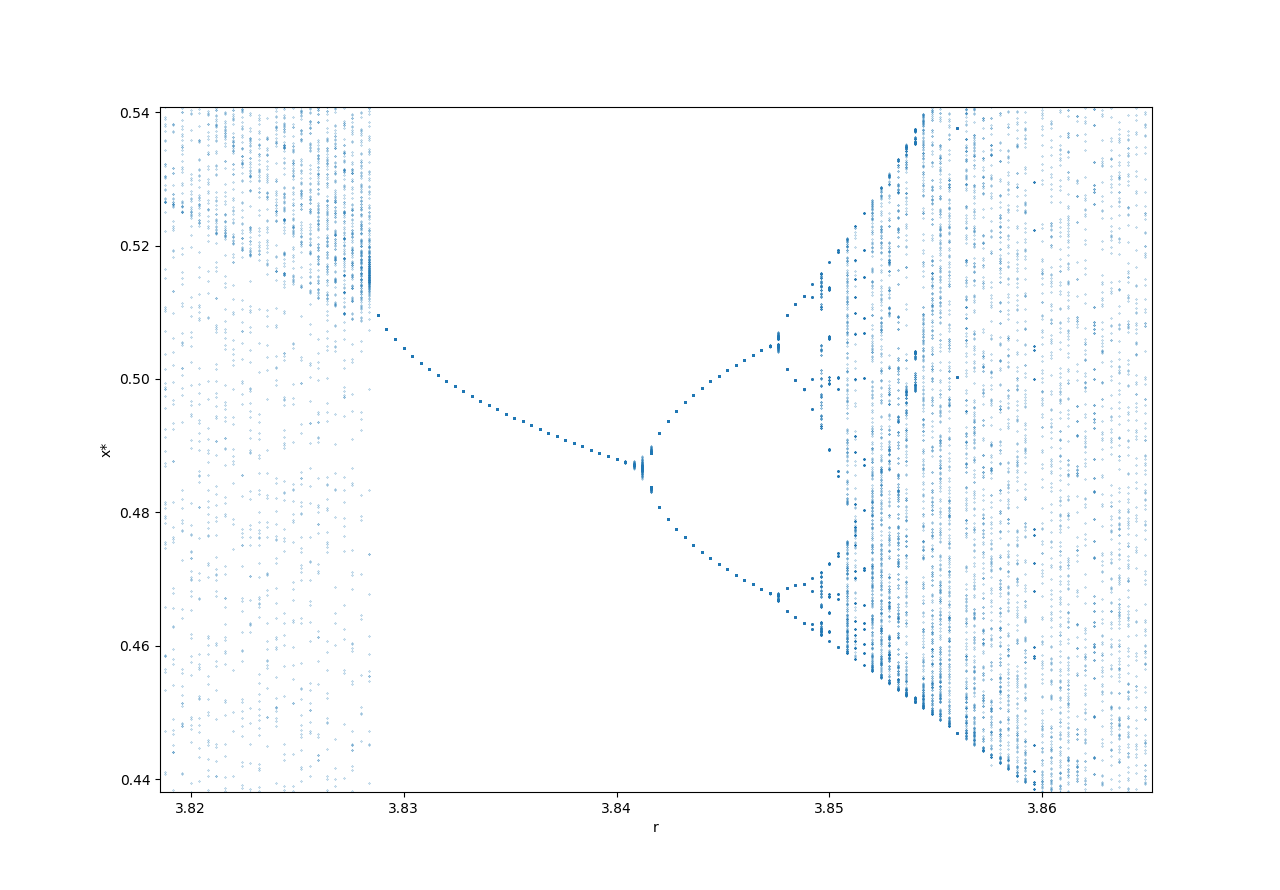
\includegraphics[scale=0.32]{/home/russo/Intro_Fiscomp/P5/2/b/frac3.png}
\caption{Zoom no diagrama.}
\label{fig 13}
\end{figure}

Embora haja uma limitação de resolução devido ao número de valores de $r$ iterados, podemos ver bem esta região ao rodarmos o código novamente com $r$ variando dentro dessa região:

\begin{figure}[H]
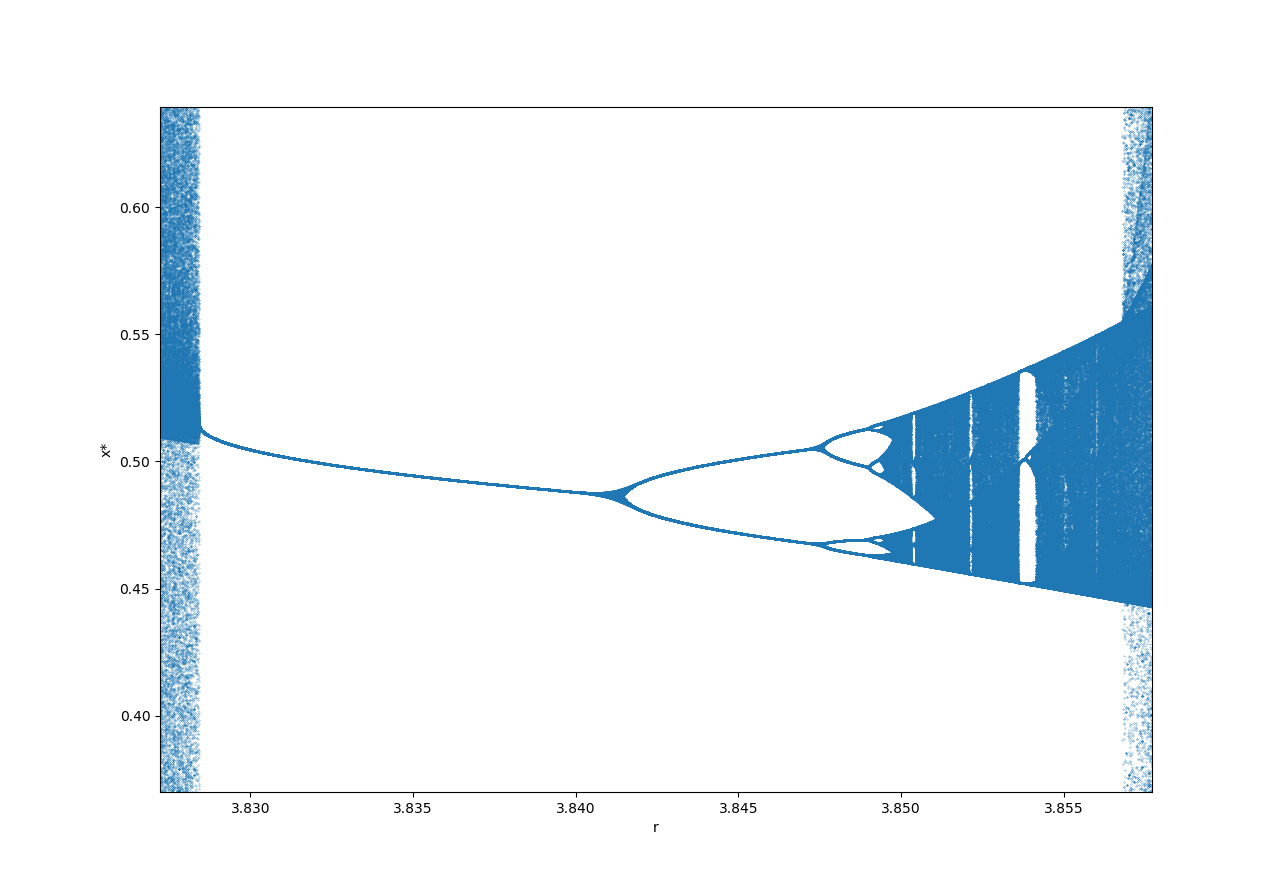
\includegraphics[scale=0.25]{/home/russo/Intro_Fiscomp/P5/2/b/frac4.png}
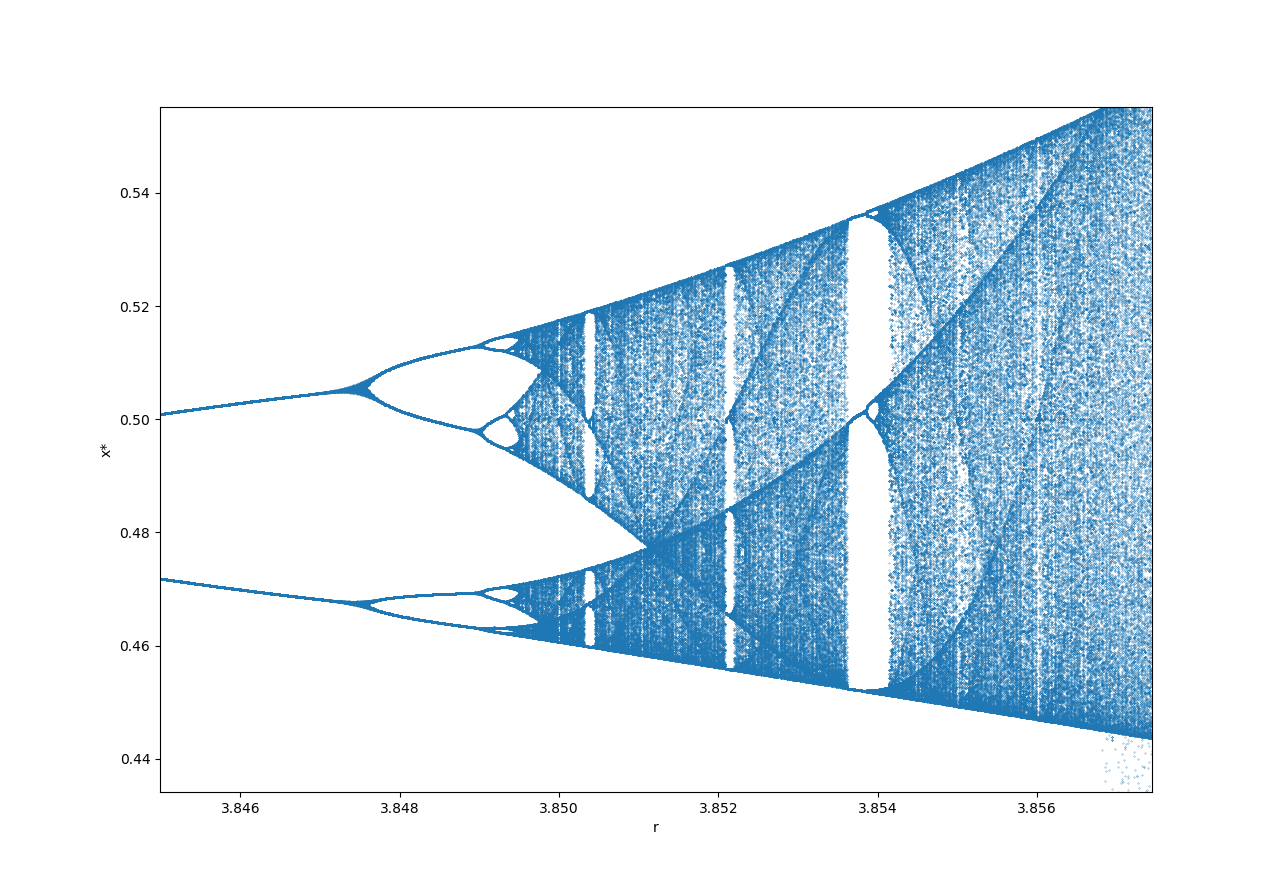
\includegraphics[scale=0.25]{/home/russo/Intro_Fiscomp/P5/2/b/frac6.png}
\caption{Iteração para novo intervalo de $r$ dentro do caos.}
\label{fig 14}
\end{figure}

\subsubsection{(c)}
\mbox{}

Usando o mesmo código, simplesmente mudo o intervalo de interação de $r$ para que $r_{2}, r_{3}$ possam ser determinados com maior precisão (sabemos que $r_{1} = 3$):

\begin{figure}[H]
\includegraphics[scale=0.25]{/home/russo/Intro_Fiscomp/P5/2/c/r2.png}
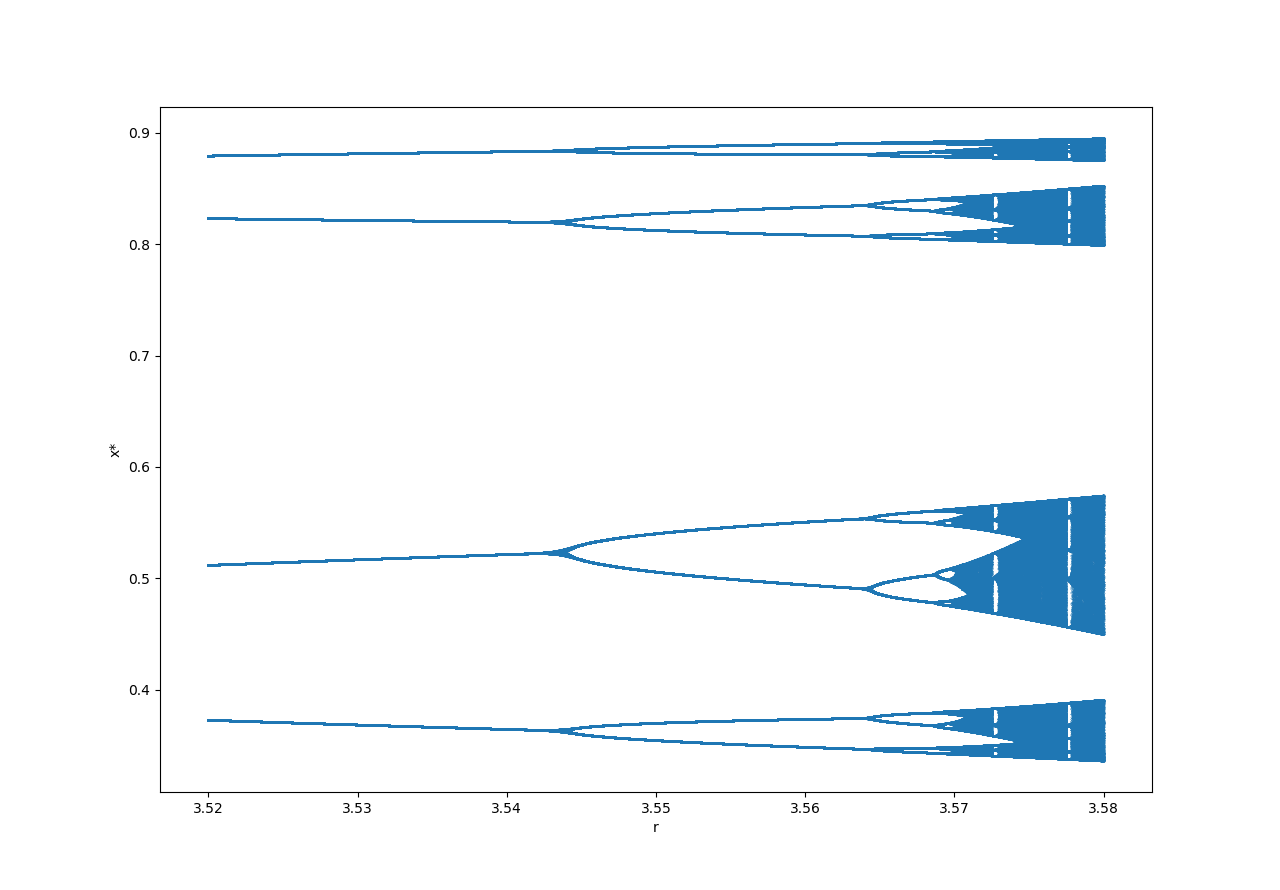
\includegraphics[scale=0.25]{/home/russo/Intro_Fiscomp/P5/2/c/r3.png}
\caption{Iteração para novo intervalo de $r$ para determinar bifurcações.}
\label{fig 15}
\end{figure}

Com os valores obtidos, podemos calcular que 

\begin{align*}
\delta = \frac{r_{2} - r_{1}}{r_{3} - r_{2}} = 4.6863
\end{align*}

é o coeficiente de Feigeinbaum.

\subsubsection{(d)}
\mbox{}

Para cinco diferentes valores de $r$ tais que $3.569946 < r < 4$ determinamos cinco valores de $x_{0}$ e um $\epsilon = 10^{-10}$. Iteramos para cada valor, $G(x_{0}, r)$ e $G(x_{0} + \epsilon, r)$ em um loop, calculando suas distâncias.

Plotando $x$ contra $i$ obtemos:

\begin{figure}[H]
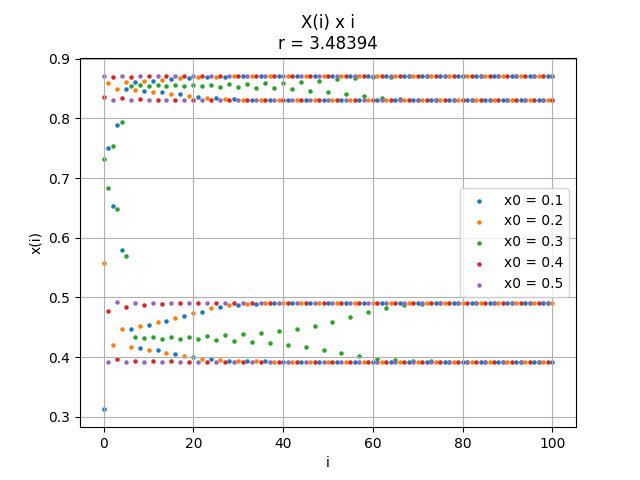
\includegraphics[scale=0.42]{/home/russo/Intro_Fiscomp/P5/2/d/xi3,4839.png}
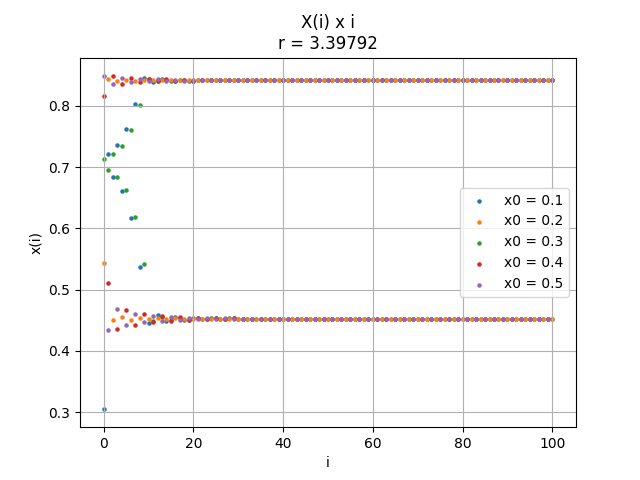
\includegraphics[scale=0.42]{/home/russo/Intro_Fiscomp/P5/2/d/xi3,3979.png}

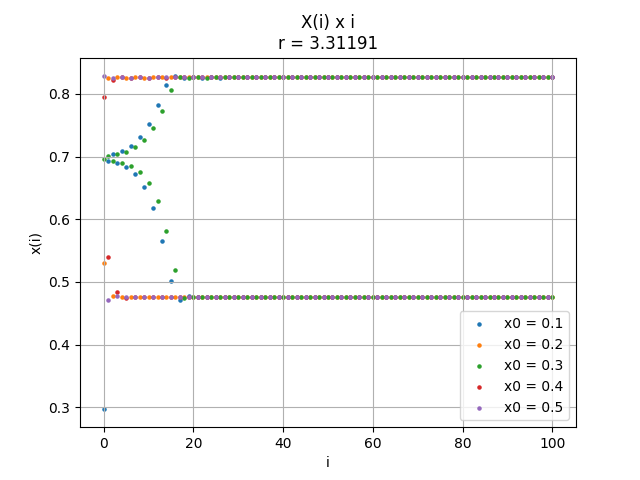
\includegraphics[scale=0.42]{/home/russo/Intro_Fiscomp/P5/2/d/xi3,3119.png}
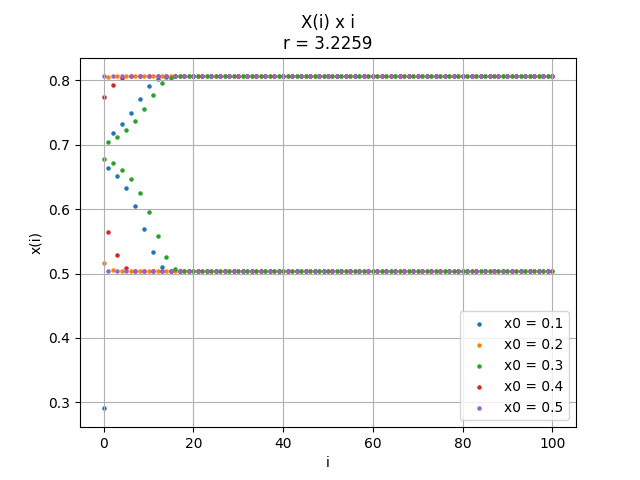
\includegraphics[scale=0.42]{/home/russo/Intro_Fiscomp/P5/2/d/xi3,2259.png}
\end{figure}
\begin{figure}[H]
\centering
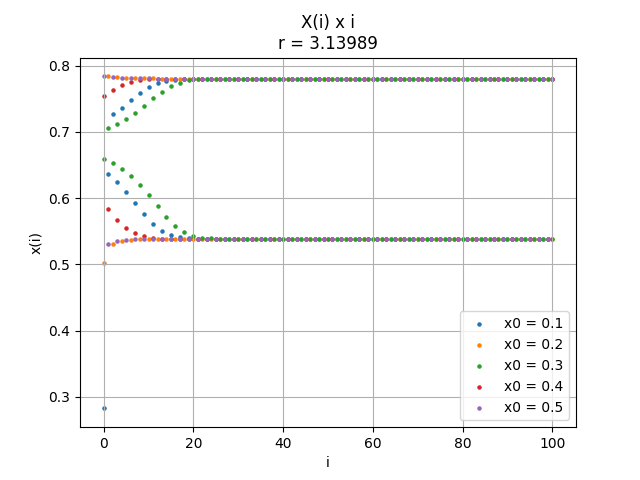
\includegraphics[scale=0.42]{/home/russo/Intro_Fiscomp/P5/2/d/xi3,1399.png}
\caption{Gráficos de $x$ contra $i$.}
\label{fig 16}
\end{figure}

Já para $d_{i}$ contra $i$:

\begin{figure}[H]
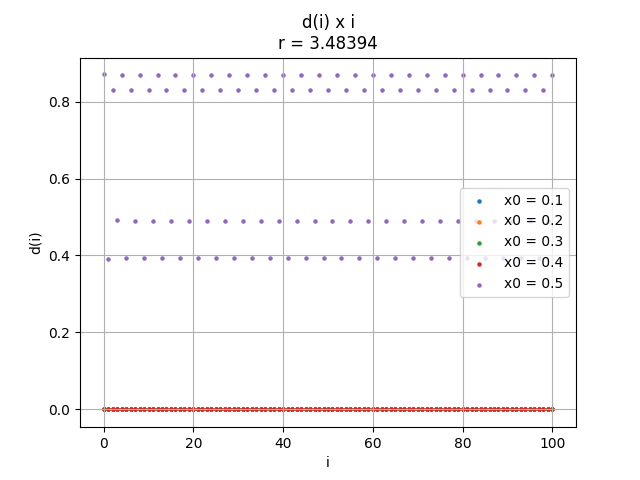
\includegraphics[scale=0.42]{/home/russo/Intro_Fiscomp/P5/2/d/Di3,4839.png}
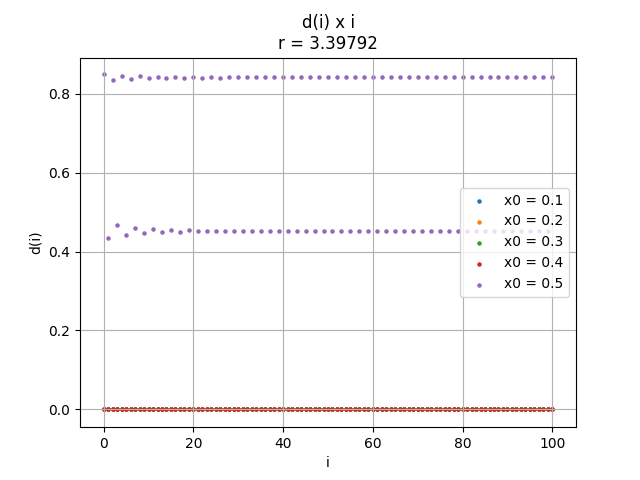
\includegraphics[scale=0.42]{/home/russo/Intro_Fiscomp/P5/2/d/Di3,3979.png}

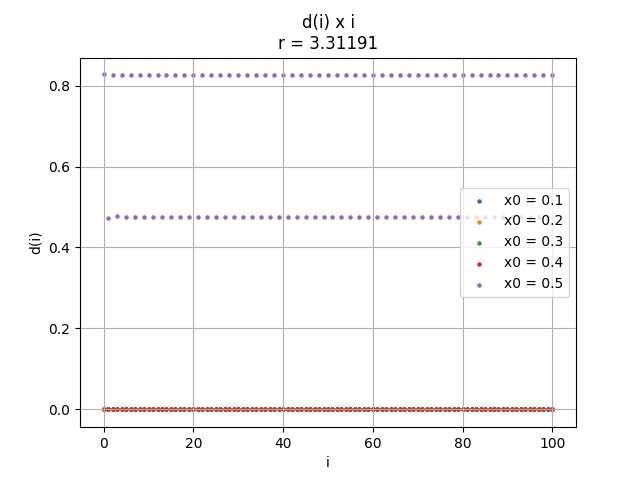
\includegraphics[scale=0.42]{/home/russo/Intro_Fiscomp/P5/2/d/Di3,3119.png}
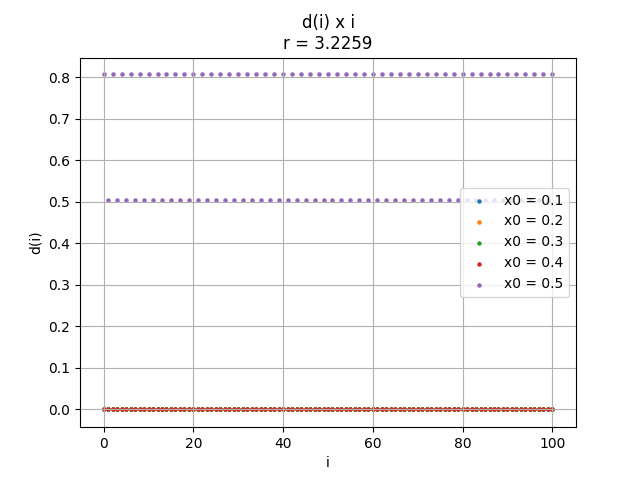
\includegraphics[scale=0.42]{/home/russo/Intro_Fiscomp/P5/2/d/Di3,2259.png}
\end{figure}
\begin{figure}[H]
\centering
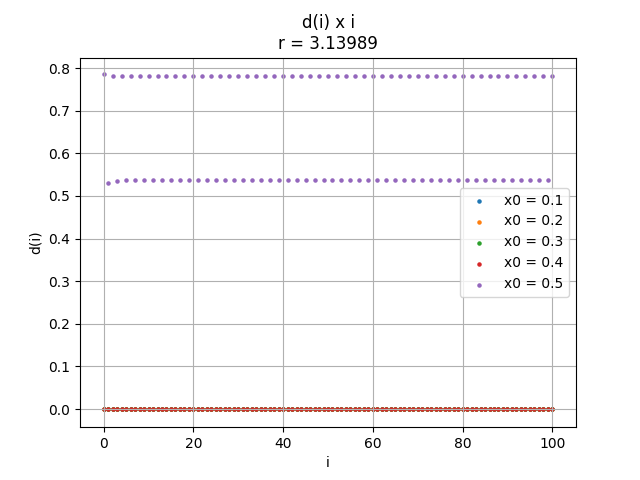
\includegraphics[scale=0.42]{/home/russo/Intro_Fiscomp/P5/2/d/Di3,1399.png}
\caption{Gráficos de $d_{i}$ contra $i$.}
\label{fig 16}
\end{figure}

Podemos ver que diferente do que foi observado no exercício anterior, $d_{i}$ se estabiliza em diferentes valores diferentes de $0$. Isso mostra que, mesmo com um $\epsilon$ muito pequeno, já é o suficiente para resultar uma grande diferença no ponto fixo. Isso é o esperado para o caos determinístico: uma pequena diferença nas condições iniciais escala rapidamente no decorrer da evolução do sistema.

\subsection{Modelo predador-presa}

\subsubsection{(a)}
\mbox{}

Levando em conta as equações:

\begin{equation}
\frac{dx}{dt} = Ax - Bxy
\end{equation}

\begin{equation}
\frac{dy}{dt} = - Cy + Dxy
\end{equation}

A constante A está relacionada com a frequência de reprodução das presas. Se definirmos que ${dx\over{dt}}$ é alguma unidade do tipo "presas por instante de tempo", para que a igualdade valha, $[A] = {1\over{tempo}}$, o que está de acordo com o esperado para uma frequência.

B, por sua vez, contribuí negativamente para a variação do número de presas. Ele está definido de tal forma que $[B] = {1\over{tempo*predador}}$. Também podemos notar que, sendo $B > A$, uma vez que $x, y > 0$ (não faria sentido termos um número negativo de animais), a população de presas decresce enquanto $y > 1$ e $x > 1$.Disso tudo, podemos deduzir que B está relacionado com a "eficiência" (ou velocidade) dos predadores em atacarem as presas.

Análogamente, as constantes C e D são definidas de forma parecida, com algumas diferenças: embora também tenha a unidade de $1\over{tempo}$, C está relacionado com o termo que contribui negativamente para a variação dos predadores. Isso porque o aparecimento de novos predadores, embora de imediato esteja contribuíndo para o aumento do número destes, em relação a variação deles no tempo, está retardando seu crescimento (já que mais predadores implica em uma competição maior pelas presas).
Quanto à D, temos que $[D] = {1\over{tempo*presa}}$, e também está relacionado com a facilidade dos predadores em obter caça.

\subsubsection{(b)}
\mbox{}

Através do método de Runge-Kutta 4, discretizamos as equações [5] e [6] de forma a obter:

\begin{align*}
f_{x}(x, y) = ax -bxy \\
f_{y}(x, y) = -cy + dxy \\
\\
F_{x}^{1} = f_{x}(x, y)\\
F_{y}^{1} = f_{y}(x, y)\\
F_{x}^{2} = f_{x}(x + 0.5*dt*F_{x}^{1}, y + 0.5*dt*F_{y}^{1})\\
F_{y}^{2} = f_{y}(x + 0.5*dt*F_{x}^{1}, y + 0.5*dt*F_{y}^{1})\\
F_{x}^{3} = f_{x}(x + 0.5*dt*F_{x}^{2}, y + 0.5*dt*F_{y}^{2})\\
F_{y}^{3} = f_{y}(x + 0.5*dt*F_{x}^{2}, y + 0.5*dt*F_{y}^{2})\\
F_{x}^{4} = f_{x}(x + 0.5*dt*F_{x}^{3}, y + 0.5*dt*F_{y}^{3})\\
F_{y}^{4} = f_{y}(x + 0.5*dt*F_{x}^{3}, y + 0.5*dt*F_{y}^{3})\\
\end{align*}

E integramos numericamente:

\begin{align*}
x_{i+1} = x_{i} + \frac{dt}{6} (F_{x}^{1} + \frac{1}{2}F_{x}^{2} + \frac{1}{2}F_{x}^{3} + F_{x}^{4})\\
y_{i+1} = y_{i} + \frac{dt}{6} (F_{y}^{1} + \frac{1}{2}F_{y}^{2} + \frac{1}{2}F_{y}^{3} + F_{y}^{4})
\end{align*}

O programa deve simplesmente iterar estar equações, nessa ordem.

\subsubsection{(c)}
\mbox{}

Aplicamos o algoritmo descrito no item anterior para as condições iniciais $x = 10, y = 2$; $x = 0, y = 2$; $x = 10, y = 0$ respectivamente. Desta forma, obtemos:

\begin{figure}[H]
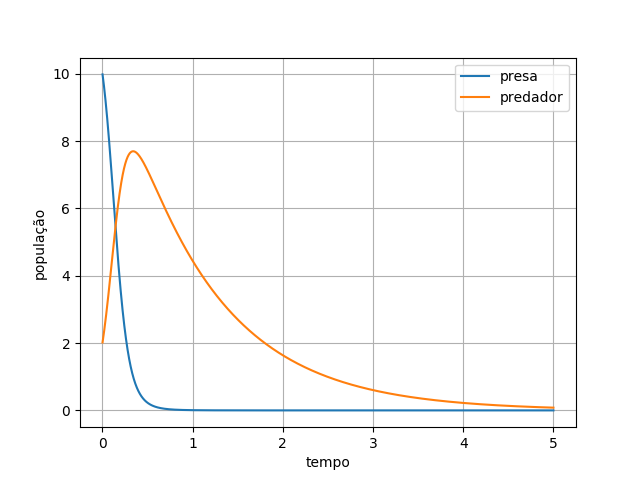
\includegraphics[scale=0.5]{/home/russo/Intro_Fiscomp/P5/3/c/popxtempo.png}
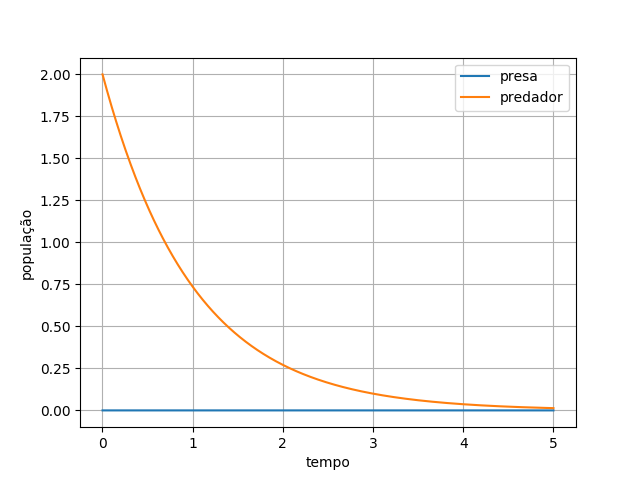
\includegraphics[scale=0.5]{/home/russo/Intro_Fiscomp/P5/3/c/presa0.png}
\end{figure}
\begin{figure}[H]
\centering
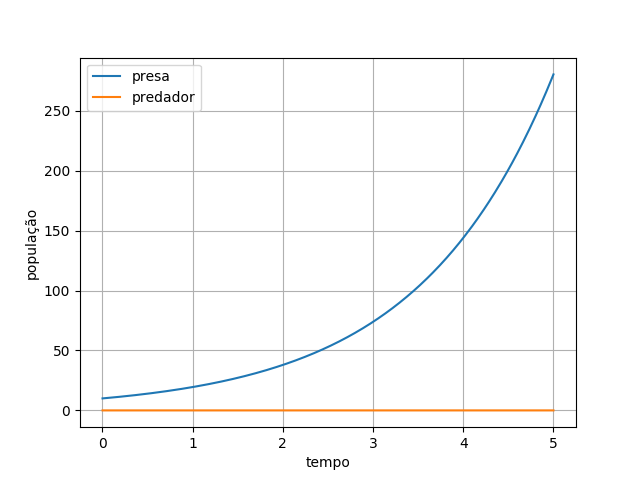
\includegraphics[scale=0.5]{/home/russo/Intro_Fiscomp/P5/3/c/predador0.png}
\caption{Dimâmica predador-presa para diferentes valores iniciais.}
\label{fig 18}
\end{figure}

Os dois últimos casos são especialmente fáceis de analisar:

Caso o número de predadores seja zero, temos:

\begin{align*}
\frac{dx}{dt} = ax \\
\Rightarrow \frac{dx}{x} = adt \\
\Rightarrow \int \frac{1}{x} dx = a \int dt \\
= \ln(x) + c_1 = at + c_2 \\
\end{align*}
\begin{equation}
\Rightarrow x(t) = \alpha e^{at}
\end{equation}

Onde $\alpha$ é o número inicial de presas (quando $t = 0$). Através de um método similar, podemos ver que $y(t)$ também é exponencial:

\begin{equation}
y(t) = \beta e^{-ct}
\end{equation}

$\beta$ o número inicial de predadores. Isso está de acordo com o que podemos observar dos gráficos.

\subsubsection{(d)}
\mbox{}

Graficando o espaço de fase para estes casos, obtemos respectivamente:

\begin{figure}[H]
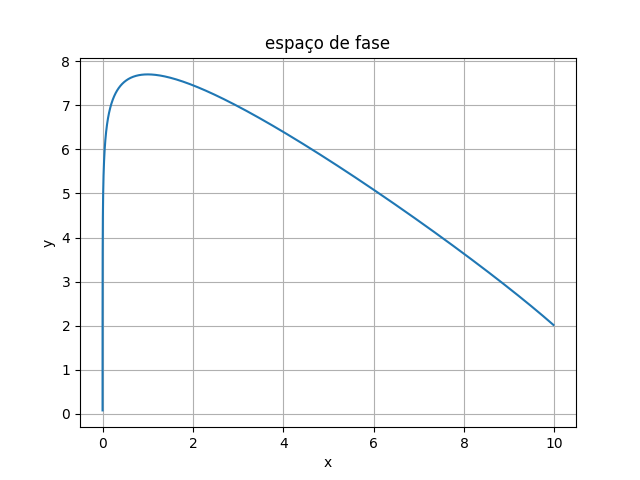
\includegraphics[scale=0.5]{/home/russo/Intro_Fiscomp/P5/3/d/efase1.png}
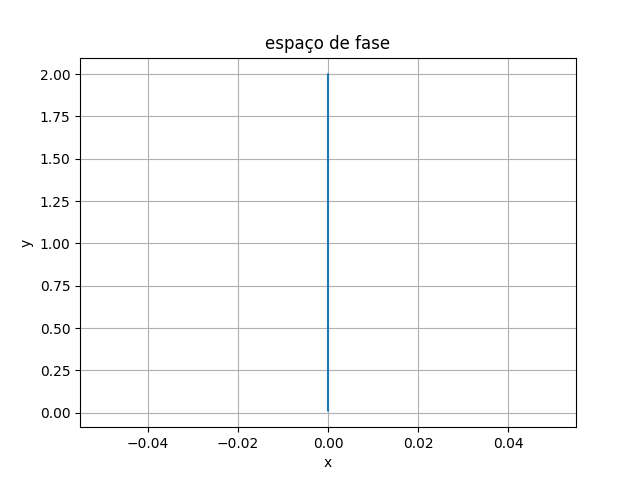
\includegraphics[scale=0.5]{/home/russo/Intro_Fiscomp/P5/3/d/efase2.png}
\end{figure}
\begin{figure}[H]
\centering
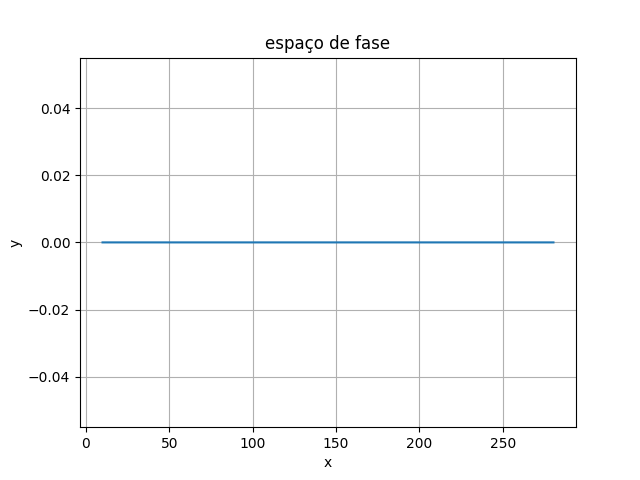
\includegraphics[scale=0.5]{/home/russo/Intro_Fiscomp/P5/3/d/efase3.png}
\caption{Espaços de fase para diferentes valores iniciais.}
\label{fig 19}
\end{figure}

\subsubsection{(e)}
\mbox{}

Dados os valores iniciais de $x, y$ e os parâmetros $a, b, c, d$ dados, plotamos o gráfico de predadores e presas por tempo, obtendo:

\begin{figure}[H]
\centering
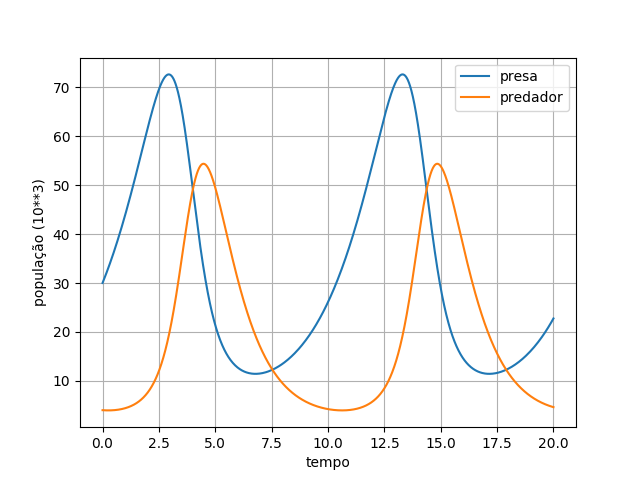
\includegraphics[scale=0.6]{/home/russo/Intro_Fiscomp/P5/3/e/popxt.png}
\caption{Predador e presa no tempo.}
\label{fig 20}
\end{figure}

E o espaço de fase:

\begin{figure}[H]
\centering
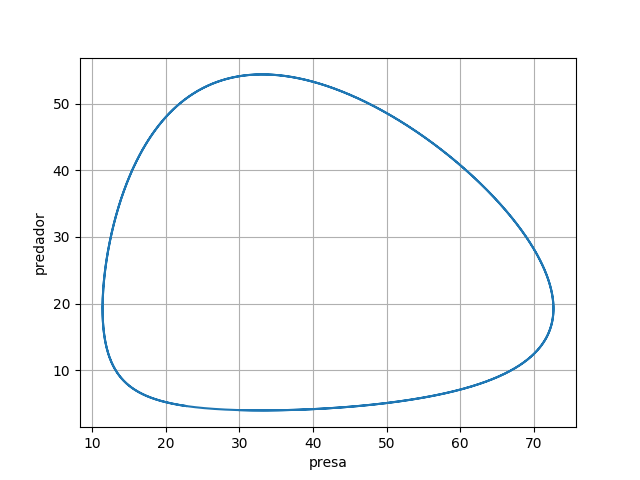
\includegraphics[scale=0.6]{/home/russo/Intro_Fiscomp/P5/3/e/presxpred.png}
\caption{Espaços de fase.}
\label{fig 21}
\end{figure}

Observando o número de lebres e linces a cada ano para comprar com a tabela fornecida, obtemos:


\begin{figure}[H]
\centering
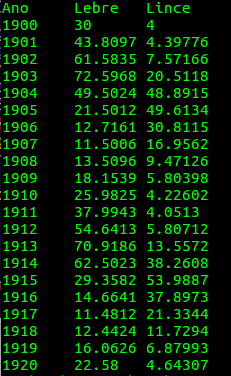
\includegraphics[scale=1]{/home/russo/Intro_Fiscomp/P5/3/e/figure.png}
\caption{Tabela com resultados dos anos.}
\label{fig 22}
\end{figure}

Embora os números sejam razoávelmente diferentes dos reais, fornecidos na tabela, o comportamento oscilatório pode ser observado nos dois casos. Se o modelo predador-presa de Lotka-Volterra é um bom modelo para esse caso, acredito que depende do propósito. Caso se deseje precisão quanto aos números brutos das populações, não é um bom modelo. Porém em relção às variações ele parece simular razoávelmente bem.

\end{document}